\chapter{Filtro Hairpin}

\section*{Resumen}
Los filtros electrónicos son circuitos que eliminan componentes de frecuencia no deseados de la señal. Suelen estar compuestos por componentes discretos (condensadores, inductores, etc.) dispuestos de forma específica para formar filtros de paso bajo, paso alto, paso banda o corte de banda. A medida que aumenta la frecuencia, esta configuración se vuelve cada vez menos fiable; los filtros de microtira son una alternativa para frecuencias más altas.

La topología de horquilla (hairpin) utiliza líneas acopladas en paralelo y se comporta como un filtro paso banda, empleado para aislar las frecuencias del ancho de banda de las señales parásitas. Ocupa relativamente poco espacio en la placa y es bastante fácil de construir en comparación con otras topologías.

\section{Aproximación de Chebyshev}

En la aproximación máximamente plana de todos los polos, se concentra el interés en $\omega=0$ y se acepta un crecimiento monótono del error para $\omega\rightarrow\infty$. Si se distribuye el error uniformemente a lo largo de la banda de paso, la función de aproximación será:

\begin{equation}
|H(j\omega)|^2 =
\frac{1}
{1+\xi^2 C_n^2\left(\dfrac{\omega}{\omega_p}\right)}
\label{eq:chebyshev_aproximacion}
\end{equation}

\begin{figure}[H]
    \centering
    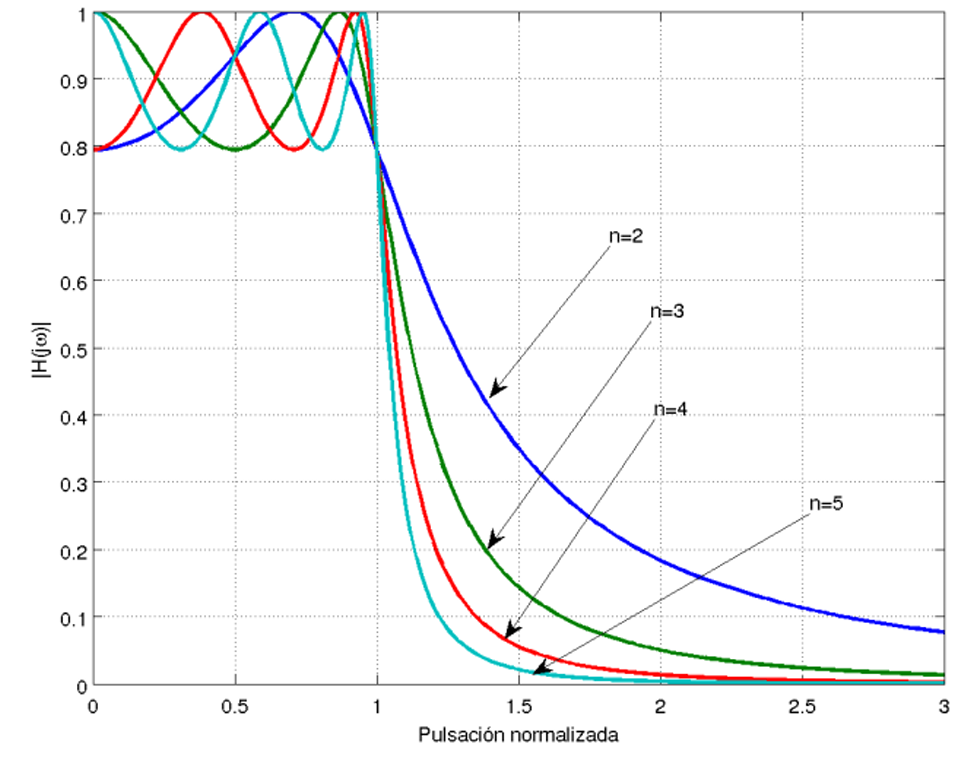
\includegraphics[width=0.5\linewidth]{imagenes/filtro_cheb.png}
    \caption{Respuesta de filtros pasabajos de Chebyshev. (Fuente: \cite{CervettoDadam2019}).}
    \label{fig:chebyshev_orden}
\end{figure}

donde $C_n$ son los polinomios de Chebyshev, que cumplen con la condición:

\begin{equation}
-1 \leq C_n\left(\frac{\omega}{\omega_p}\right) \leq 1,
\qquad
\forall \; 0 \leq |\omega| \leq \omega_p,
\end{equation}

por lo que la función oscila armónicamente entre $1$ y $(1+\xi^2)^{-1}$. Los polinomios de Chebyshev se calculan iterativamente mediante:

\begin{equation}
C_{n+1}(x) = 2x C_n(x) - C_{n-1}(x),
\end{equation}

sabiendo que:

\begin{equation}
C_0(x) = 1,
\qquad
C_1(x) = x.
\end{equation}

El orden del filtro $n$ y el coeficiente $\xi$ dependen de los parámetros de diseño. El orden del filtro se determina mediante:

\begin{equation}
n =
\frac{
\operatorname{arcosh}
\left(
\sqrt{\dfrac{10^{0.1\alpha_a}-1}
{10^{0.1\alpha_p}-1}}
\right)
}{
\operatorname{arcosh}\left(\dfrac{\omega_a}{\omega_p}\right)
},
\label{eq:orden_chebyshev}
\end{equation}

mientras que el coeficiente de rizado se obtiene como:

\begin{equation}
\xi^2 = 10^{0.1\alpha_p} - 1.
\label{eq:xi_chebyshev}
\end{equation}

Los filtros de Chebyshev directos presentan un rizado constante en la banda de paso y una función de atenuación que decrece monótonamente para $\omega \geq \omega_p$. El orden del filtro influye en la atenuación; sin embargo, la atenuación en la frecuencia de paso es independiente del orden y está dada por:

\begin{equation}
\alpha(\omega_p) = \alpha_p.
\end{equation}

Para filtros de orden par, la atenuación en $\omega=0$ es $\alpha(0)=0$, mientras que para filtros de orden impar se cumple $\alpha(0)=\alpha_p$.

En la Figura~\ref{fig:chebyshev_orden} se pueden observar las distintas respuestas obtenidas al aumentar el orden del filtro para una respuesta pasabajos normalizada \cite{CervettoDadam2019}.

\section{Diseño de filtro Hairpin}
Para el diseño del filtro se seguirá el desarrollo de A. Hasan \cite{A Hasan}, utilizando las ecuaciones de diseño correspondientes a resonadores de media longitud de onda ($\lambda/2$) acoplados en paralelo. Para plegar los resonadores, es necesario tener en cuenta la reducción de la longitud de las líneas acopladas, ya que esta disminuye el acoplamiento entre los resonadores. Los brazos de cada resonador tipo hairpin actúan como un par de líneas acopladas cuando se encuentran muy próximos entre sí.

Se debe elegir el orden del filtro y el tipo de respuesta (como Chebyshev, Butterworth, inverso de Chebyshev, etc.), además del rizado de la banda de paso y la frecuencia de corte.

Una vez elegido el filtro, se seleccionan los coeficientes del prototipo paso bajo. Para un filtro Chebyshev, se procedería de la siguiente manera:
\begin{align}
g_0 &= 1, \\
g_1 &= \frac{2a_1}{\gamma}, \\
g_k &= \frac{4a_{k-1}a_k}{b_{k-1}g_{k-1}}, \qquad k=2,3,\ldots,n, \\
g_{n+1} &= 1 \qquad \text{para } n \text{ impar}, \\
g_{n+1} &= \coth^2\left(\frac{\beta}{4}\right) \qquad \text{para } n \text{ par}.
\end{align}
\begin{align}
a_k &= \sin\left(\frac{(2k-1)\pi}{2n}\right), \qquad k=1,2,\ldots,n, \\
b_k &= \gamma^2+\sin^2\left(\frac{k\pi}{n}\right), \qquad k=1,2,\ldots,n, \\
\beta &= \ln\left[\coth\left(\frac{A}{2\times 8.686}\right)\right], \\
\gamma &= \sinh\left(\frac{\beta}{2n}\right).
\end{align}
donde $A$ es el rizado en la banda de paso expresado en decibelios:
\begin{equation}
A = 10\log_{10}\left(1+\varepsilon^2\right).
\end{equation}

\begin{equation}
\varepsilon = \sqrt{10^{A/10}-1}.
\end{equation}

Dependiendo del orden del filtro, la resistencia de terminación puede ser diferente de la resistencia de la fuente. Los parámetros de diseño del filtro pasabanda, representados por el factor de calidad externo $Q_e$, se calculan mediante:

\begin{align}
Q_{e1} &= \frac{g_0g_1}{\mathrm{FBW}}, \\
Q_{en} &= \frac{g_ng_{n+1}}{\mathrm{FBW}},
\end{align}

donde $Q_{e1}$ y $Q_{en}$ son los factores de calidad externos de los resonadores de entrada y salida, respectivamente, y $\mathrm{FBW}$ representa el ancho de banda fraccional.

\subsection{Impedancias de Modo Par e Impar}
La interacción electromagnética entre los resonadores adyacentes se modela clásicamente mediante inversores de admitancia $J_{j,j+1}$. Estos inversores determinan el grado de acoplamiento necesario para alcanzar el ancho de banda fraccional (FBW) deseado. Los valores de los inversores escalados a la admitancia característica $Y_0$ se definen como \cite{pozar}:

\begin{align}
\frac{J_{0,1}}{Y_0} &= \sqrt{\frac{\pi \cdot \mathrm{FBW}}{2 g_0 g_1}} \\
\frac{J_{j,j+1}}{Y_0} &= \frac{\pi \cdot \mathrm{FBW}}{2 \sqrt{g_j g_{j+1}}}, \qquad j = 1, 2, \ldots, n-1 \\
\frac{J_{n,n+1}}{Y_0} &= \sqrt{\frac{\pi \cdot \mathrm{FBW}}{2 g_n g_{n+1}}}
\end{align}

Dado que los brazos de los resonadores en microtira interactúan a través de campos eléctricos y magnéticos superpuestos, la propagación se descompone en un modo par (excitación simétrica) y un modo impar (excitación asimétrica). A partir de los inversores de admitancia, las impedancias características de modo par ($Z_{0e}$) e impar ($Z_{0o}$) para cada sección acoplada se calculan mediante:

\begin{align}
Z_{0e, j,j+1} &= \frac{1}{Y_0} \left[ 1 + \frac{J_{j,j+1}}{Y_0} + \left(\frac{J_{j,j+1}}{Y_0}\right)^2 \right] \\
Z_{0o, j,j+1} &= \frac{1}{Y_0} \left[ 1 - \frac{J_{j,j+1}}{Y_0} + \left(\frac{J_{j,j+1}}{Y_0}\right)^2 \right]
\end{align}

Estas impedancias son los parámetros fundamentales que, junto con las propiedades del sustrato (permitividad relativa $\varepsilon_r$ y altura $h$), permiten sintetizar el ancho físico de las pistas ($W$) y la separación entre resonadores ($S$).

Estas horquillas ubicadas muy próximas interactúan electromagnéticamente estableciendo un coeficiente de acoplamiento teórico entre ellos:
\begin{equation}
k_{jk} = \frac{\mathrm{FBW}}{\sqrt{g_j g_k}}
\end{equation}

Si la separación entre los resonadores es lo suficientemente pequeña, estos interactúan entre sí y aparecen dos frecuencias de resonancia en el parámetro de transmisión $S_{21}$. El coeficiente de acoplamiento puede calcularse en simulación mediante la siguiente expresión:
\begin{equation}
k = \frac{f_2^2 - f_1^2}{f_2^2 + f_1^2}
\end{equation}

\subsection{Alimentación por Conexión Directa}
En la topología de líneas acopladas estándar, el primer y último resonador se acoplan a los puertos de entrada y salida mediante una brecha capacitiva. Sin embargo, para filtros con anchos de banda fraccionales estrechos o moderados, el valor requerido de $Q_e$ exige una separación física extremadamente pequeña, lo que dificulta su manufactura y aumenta los costos \cite{HongLancaster}.

Para mitigar este problema en los filtros hairpin, se emplea una técnica de alimentación por línea con derivación (\textit{tapped-line}). En esta configuración, la línea de alimentación de $50\,\Omega$ se conecta físicamente de forma directa al primer y último resonador. 

El factor de calidad externo $Q_e$ queda determinado por la posición física de la conexión en el resonador. La distancia $L_t$ desde el centro virtual de cortocircuito (la base de la U del hairpin) hasta el punto de derivación se aproxima mediante la expresión:

\begin{equation}
L_t = \frac{\lambda_g}{2\pi} \arcsin\left( \sqrt{ \frac{\pi}{2} \frac{Z_0}{Z_r Q_e} } \right)
\end{equation}

donde $\lambda_g$ es la longitud de onda guiada a la frecuencia central, $Z_0$ es la impedancia característica de la línea de alimentación, y $Z_r$ es la impedancia característica del resonador. Esta técnica elimina la dependencia de una brecha de acoplamiento crítica, trasladando el ajuste del $Q_e$ a la longitud $L_t$, un parámetro mucho más controlable en el proceso de fabricación.

\subsection{Consideraciones Topológicas y Simulación Electromagnética}
La topología hairpin impone desafíos adicionales frente a los resonadores rectos de media onda ($\lambda/2$). Al plegar el resonador para formar la característica forma de U, se introducen discontinuidades físicas. La principal consideración geométrica exige que la separación entre los dos brazos del \textit{mismo} resonador sea lo suficientemente amplia para minimizar el auto-acoplamiento (capacitancia parásita interna), lo cual degradaría el factor de calidad no descargado ($Q_u$).

Dado que el acoplamiento final depende de una función compleja no lineal que involucra el ancho de la línea $W$, la separación $S$, la longitud de acoplamiento, el espesor del sustrato $h$ y la constante dieléctrica $\varepsilon_r$, las ecuaciones analíticas proporcionan únicamente un modelo inicial. Para centrar la frecuencia de operación y compensar los efectos parasitarios de las curvas y uniones en T de la alimentación, es imperativo exportar la síntesis geométrica a un simulador electromagnético de microondas. Mediante un análisis de método de momentos (MoM), se realiza un barrido paramétrico optimizando iterativamente las dimensiones físicas hasta obtener la respuesta de parámetros S deseada \cite{A Hasan}.

\begin{figure}[H]
    \centering
    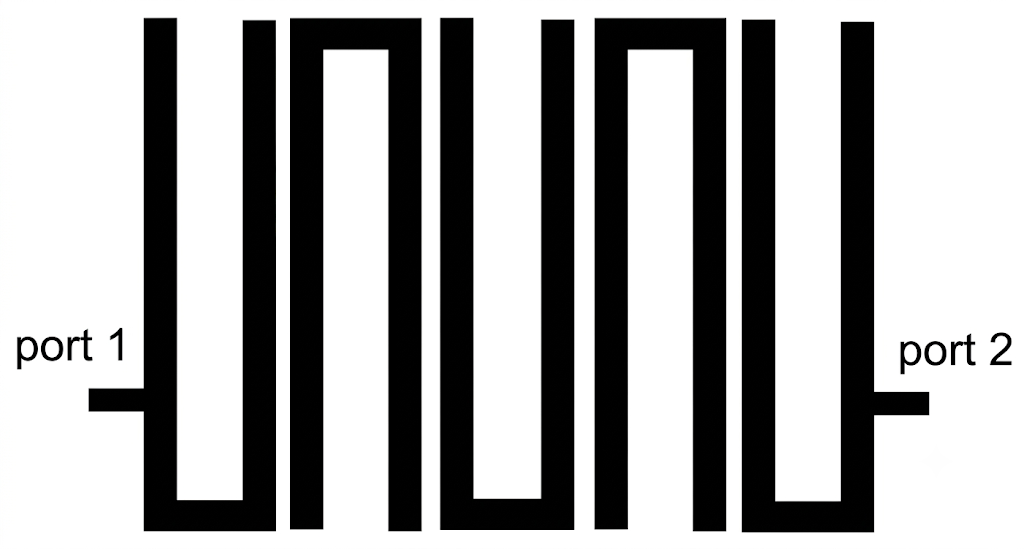
\includegraphics[width=0.75\linewidth]{imagenes/hairpin.png}
    \caption{Filtro pasabanda Hairpin de 5to orden. (Fuente: \cite{A Hasan}).}
    \label{fig:hairpin_5to_orden}
\end{figure}